\documentclass[cameraready]{Interspeech}
\usepackage{float}
\usepackage{amsmath}
\usepackage{amssymb}
\usepackage{hyperref}
\usepackage{graphicx}
\usepackage{tabularx}
\usepackage{booktabs}
\usepackage{array}
\usepackage{enumitem}
\usepackage{tikz}
\usetikzlibrary{arrows.meta,positioning,shapes.geometric}

\title{Decentralised Weather Mesh Networking for Maritime Safety:\\
       A Multi-Agent Simulation Study}

\author[affiliation={1}]{Pawe\l}{Pozorski}
\author[affiliation={1}]{Micha\l}{Pytel}

\address{$^1$ Warsaw University of Technology, Poland}

\email{\{pawel.pozorski, michal.pytel\}.stud@pw.edu.pl}

\keywords{maritime safety, multi-agent systems, agent-based modelling,
decentralised communication, human factors, collision avoidance}

\begin{document}

\maketitle

% ------------------------------------------------------------------
\begin{abstract}
Between 70--96\,\% of maritime casualties involve human error~\cite{imohuman2018}; weather uncertainty compounds this when vessels lose shore radio coverage. Shore broadcasts carry Gaussian noise, cannot resolve localised storm cells, and leave vessels in radio shadows entirely uninformed. We model a decentralised ship-to-ship weather mesh in which vessels exchange local observations via a hop-limited gossip protocol, blending them with shore forecasts through confidence-weighted fusion. A preparedness score coupling forecast accuracy and crew fatigue gates all tactical decisions, including early evacuation. Against a classical and a shore-only baseline, the system is tested across four adversarial scenarios in a Mesa agent-based simulation with 30 seed-matched runs per condition. We hypothesise that the mesh will reduce the fatal event rate by at least ${\geq}20\,\%$ and improve post-collision survival by at least ${\geq}15\,\%$; the gains are expected to hold even when shore forecast noise doubles and all vessels operate beyond the $50$\,nm coastal radio horizon.
\end{abstract}

% ==================================================================
\section{Introduction}
\label{sec:intro}
% ==================================================================

Maritime transport carries roughly 80\,\% of global trade, yet the sector's safety record is dominated by a persistent human-error problem. The International Maritime Organization (IMO) attributes 70--96\,\% of all incidents to human causes~\cite{imohuman2018}, and the European Maritime Safety Agency (EMSA) identifies weather as a compounding factor in a disproportionate share of total-loss events, particularly in congested coastal corridors where crew fatigue and information latency interact~\cite{emsa2023}. Hull and machinery insurance claims exceed USD 3.5\,billion annually~\cite{iumi2023}; even a 5\,\% reduction in fatal incidents would yield hundreds of millions in avoided liability.

The International Regulations for Preventing Collisions at Sea (COLREGs)~\cite{colregs1972} provide a deterministic collision-avoidance baseline whose implicit assumption — that crews have accurate, timely situational awareness — fails under three compounding conditions that prior agent-based maritime simulation literature~\cite{tam2010,silveira2013,zhang2015}
has not addressed jointly:

\begin{itemize}
    \item \textbf{Imperfect weather-information flow.} Existing simulation models grant vessels omniscient access to the true weather field. In practice, shore broadcasts are noisy and range-limited; vessels beyond the coastal horizon have no external weather source at all.

    \item \textbf{Human-factor coupling.} Crew fatigue accumulates over watch cycles and follows a circadian pattern with a late-night performance nadir~\cite{chauvin2013}. Prior models isolate fatigue in peripheral sub-models without direct connection to tactical decision logic.

    \item \textbf{Cross-vessel survival and rescue logistics.} Evacuation timing and rescue Time-to-Arrival (TTA) are rarely co-modelled; the survival payoff of early, well-informed preparedness therefore cannot be quantified~\cite{goerlandt2014}.
\end{itemize}


The contribution of this work is a \emph{ship-to-ship weather mesh network} grounded in epidemic broadcast theory~\cite{demers1987} and decentralised maritime navigation research~\cite{naus2016}. Vessels relay local weather observations to neighbours via a two-hop gossip protocol, bridging radio shadows and compensating for shore forecast degradation. Fatigue and circadian phase are embedded directly in a preparedness score that governs every manoeuvre and evacuation decision, creating a quantified causal link from \emph{information quality} to \emph{crew survival}.

% ==================================================================
\section{Research Objectives}
\label{sec:goal}
% ==================================================================

The central thesis is: \emph{decentralised ship-to-ship weather mesh networking, coupled with human-factor-aware preparedness scoring, reduces fatal maritime outcomes more effectively than centralised shore-broadcast systems alone.}

\begin{description}
    \item[Experimental conditions.] All experiments compare three methods:
        \begin{description}[leftmargin=2.2em, labelindent=0pt]
            \item[Baseline~A (Classical)] represents current practice: vessels follow COLREGs with no weather intelligence and no preparedness modifier.
            \item[Baseline~B (Shore-Only)] adds reception of coastal-station broadcasts when in range, but has no peer relay and no confidence-weighted fusion.
            \item[Proposed System] integrates the full decentralised mesh — hop-limited relay, confidence-weighted forecast fusion, adaptive shore-trust decay, preparedness scoring, early evacuation, and SOS relay — all described formally in Sections~\ref{sec:comms} and~\ref{sec:behaviour}. Performance is measured using six KPIs defined in Table~\ref{tab:kpis}.
        \end{description}

    \item[Falsifiable hypotheses.] They drive all design decisions; any component that contributes to none of them is excluded.
        \begin{description}[leftmargin=2.2em, labelindent=0pt]
            \item[\textbf{H1.}] Enabling the mesh reduces the fatal event rate (Table~\ref{tab:kpis}, KPI~1) by ${\geq}20\,\%$ versus Baseline~A ($p < 0.05$, Mann-Whitney U, Cliff's $\Delta > 0.2$).
            \item[\textbf{H2.}] Early mesh-informed evacuation improves post-collision survival (Table~\ref{tab:kpis}, KPI~3) by ${\geq}15\,\%$ versus Baseline~A.
            \item[\textbf{H3.}] The Proposed System outperforms Baseline~B on fatal event rate ($p < 0.05$) even when shore forecast standard deviation doubles and vessel initialisation is constrained to endpoint-centred offshore spawn annuli.
        \end{description}

\end{description}

% ==================================================================
\section{System Model}
\label{sec:model}
% ==================================================================

\subsection{World Geometry and Time Resolution}

The simulation occupies a $100 \times 100$\,nm continuous space built on the Mesa agent-based modelling framework~\cite{mesa2020}. A static land mask defines an island-archipelago geometry: an irregular western mainland with distributed offshore islands and shallow banks. Five intersecting non-linear waypoint routes cover the navigable area — three west-east corridors (\texttt{west\_east\_southern}, \texttt{west\_east\_mid\_channel}, \texttt{west\_east\_northern\_arc}) and two north-south channels (\texttt{north\_south\_west\_channel}, \texttt{north\_south\_central\_channel}). All five are validated at startup against shore-proximity, shoreline-clearance, and boundary conditions, so the default configuration requires no manual repair.

Shipping lanes are ordered waypoint polylines; segments intersecting land are rejected at load time. The model supports one or more coastal stations, each placed on land, broadcasting with radius $R_\text{shore} = 50$\,nm. The default single station sits at $(0, 50)$\,nm on the western mainland. Vessels spawn at a point drawn from an annulus centred on a sampled route endpoint, with bounds $[r_\text{min}, r_\text{max}]$ and a radial bias toward the outer ring.

Time advances in discrete \emph{macro ticks} of 15\,min ($\Delta t = 0.25$\,hr). Within each tick, computation runs in four ordered phases: weather update, shore broadcast and relay, agent behaviour, and post-step physics with housekeeping (see Section~\ref{sec:loop}). All stochastic draws use a single seeded RNG, so identical seeds reproduce byte-identical KPI logs.

\subsection{Agent Types}

The system relies on three agent types:

\begin{description}
    \item[Vessel agents] traverse shipping lanes as ordered waypoint sequences (not nearest-point shortcuts), enabling non-linear route geometry. Each maintains position, heading, speed, and crew archetype (Veteran / Standard / Green), together with accumulated fatigue (\texttt{hours\_awake}), a local weather observation at the vessel's current cell, a radio inbox of received mesh packets, and a preparedness score $P_\text{prep}$ (Section~\ref{sec:behaviour}) that gates all tactical decisions. Speed is drawn at spawn from $\mathcal{U}(10, 20)$\,kn and reduced each tick by the hazard slowdown factor $\max(0.30,\,1 - 0.45\,W)$, so vessels in maximum hazard travel at 30\,\% of their nominal speed. Each vessel carries $n_\text{crew} = 10$ survivors; structural integrity has a \texttt{stability\_threshold} of~3 damage points — reached by three collision or grounding events — after which the vessel transitions directly to \texttt{SUNK}. State transitions follow: \texttt{ACTIVE} $\to$ \texttt{EVAC} $\to$ \texttt{SUNK} or \texttt{RESCUED}.

    \item[Coastal station agents] are stationary. Each tick they sample the true weather at their position, add Gaussian forecast noise (Eq.~\ref{eq:shoreNoise}), and broadcast to vessels satisfying the receive probability criterion (Eq.~\ref{eq:Prx}). Distress signals are probabilistically received by shore stations using the same radio model; rescue assets are spawned from the station that successfully received the SOS, not from a globally fixed origin.

    \item[Rescue agents] are spawned on SOS dispatch. The engine draws the asset type with equal probability: helicopter (80\,kn) or patrol vessel (25\,kn)~\cite{imosar2018}. Both asset types undergo a weather-dependent speed penalty, $v_\text{eff} = v \cdot \max(0.40,\,1 - 0.35\,W)$, so severe conditions reduce transit speed by up to 60\,\%. Asset mobilisation requires $\Delta t_\text{mob} = 2$ ticks before movement begins. On arrival at the distress position (within 0.2\,nm), surviving crew members transition to \texttt{RESCUED} and the \texttt{survival\_ratio} counter increments (Table~\ref{tab:kpis}, KPI~3). Rescue assets carry no fatigue model, have unlimited capacity, and are never lost to the environment.
\end{description}

Fig.~\ref{fig:classes} summarises the ownership relationships among all five component types.

\begin{figure*}[t]
\centering
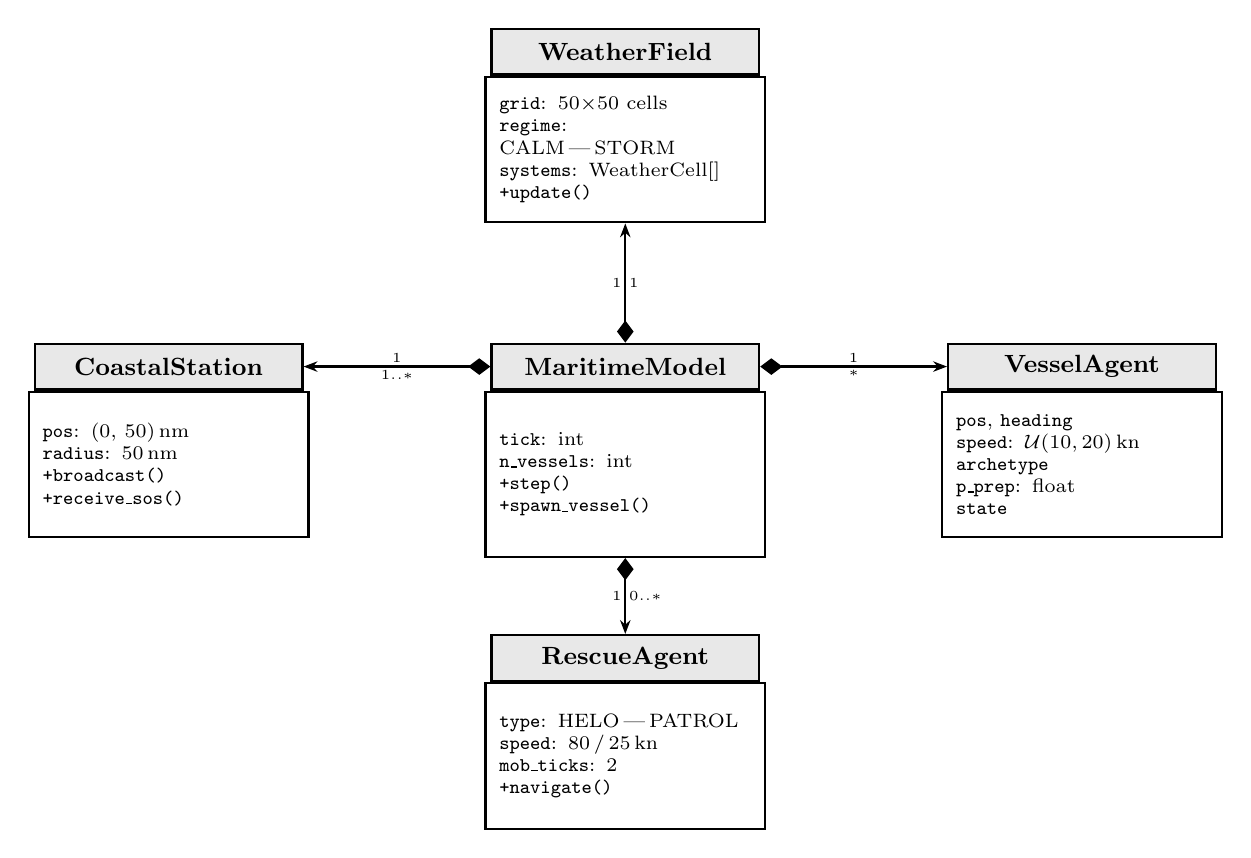
\begin{tikzpicture}[
  >=Stealth,
  hdr/.style={draw, thick, fill=gray!18,
              minimum width=3.4cm, minimum height=0.58cm,
              align=center, font=\small\bfseries, inner sep=3pt},
  bdy/.style={draw, thick,
              minimum width=3.4cm, minimum height=1.85cm,
              align=left, inner sep=5pt, text width=3.2cm, font=\scriptsize},
  lbl/.style={font=\tiny, fill=white, inner sep=1pt},
]
  %% WeatherField — top centre
  \node[hdr] (wf_h) at (0, 6.5)   {WeatherField};
  \node[bdy, anchor=north] (wf) at (wf_h.south) {
    \texttt{grid}: 50$\times$50 cells\\
    \texttt{regime}: CALM\,|\,STORM\\
    \texttt{systems}: WeatherCell[]\\
    \texttt{+update()}
  };

  %% MaritimeModel — centre
  \node[hdr] (mm_h) at (0, 2.5)   {MaritimeModel};
  \node[bdy, anchor=north, minimum height=2.1cm] (mm) at (mm_h.south) {
    \texttt{tick}: int\\
    \texttt{n\_vessels}: int\\
    \texttt{+step()}\\
    \texttt{+spawn\_vessel()}
  };

  %% CoastalStation — left
  \node[hdr] (cs_h) at (-5.8, 2.5) {CoastalStation};
  \node[bdy, anchor=north] (cs) at (cs_h.south) {
    \texttt{pos}: $(0,\,50)$\,nm\\
    \texttt{radius}: 50\,nm\\
    \texttt{+broadcast()}\\
    \texttt{+receive\_sos()}
  };

  %% VesselAgent — right
  \node[hdr] (va_h) at (5.8, 2.5)  {VesselAgent};
  \node[bdy, anchor=north] (va) at (va_h.south) {
    \texttt{pos}, \texttt{heading}\\
    \texttt{speed}: $\mathcal{U}(10,20)$\,kn\\
    \texttt{archetype}\\
    \texttt{p\_prep}: float\\
    \texttt{state}
  };

  %% RescueAgent — bottom centre
  \node[hdr] (ra_h) at (0, -1.2)  {RescueAgent};
  \node[bdy, anchor=north] (ra) at (ra_h.south) {
    \texttt{type}: HELO\,|\,PATROL\\
    \texttt{speed}: 80\,/\,25\,kn\\
    \texttt{mob\_ticks}: 2\\
    \texttt{+navigate()}
  };

  %% Composition arrows: filled diamond at MaritimeModel, arrowhead at component
  \draw[thick, {Diamond[fill=black,length=8pt,width=6pt]}-{Stealth[length=5pt]}]
    (mm_h.north) -- node[lbl,left]{1} node[lbl,right]{1} (wf.south);
  \draw[thick, {Diamond[fill=black,length=8pt,width=6pt]}-{Stealth[length=5pt]}]
    (mm_h.west)  -- node[lbl,above]{1} node[lbl,below]{$1..*$} (cs_h.east);
  \draw[thick, {Diamond[fill=black,length=8pt,width=6pt]}-{Stealth[length=5pt]}]
    (mm_h.east)  -- node[lbl,above]{1} node[lbl,below]{$*$} (va_h.west);
  \draw[thick, {Diamond[fill=black,length=8pt,width=6pt]}-{Stealth[length=5pt]}]
    (mm.south)   -- node[lbl,left]{1} node[lbl,right]{$0..*$} (ra_h.north);
\end{tikzpicture}
\caption{UML class diagram of the core simulation components. Filled diamonds denote composition: \texttt{MaritimeModel} exclusively owns one \texttt{WeatherField}, at least one \texttt{CoastalStation}, an arbitrary fleet of \texttt{VesselAgent}s, and zero or more \texttt{RescueAgent}s spawned on demand. Multiplicities are shown at each arrow end.}
\label{fig:classes}
\end{figure*}

\subsection{Weather Field}

A $50 \times 50$-cell grid evolves with a Tier-2 stochastic process designed to produce realistic mesoscale structure: calm/storm regime switching, moving circular systems, coherent fronts, and bounded random shocks. The process is updated each macro tick and remains seed-deterministic for exact replay. Three physical channels --- sea state, visibility, and wind intensity --- are evolved jointly, then combined into a single normalised hazard scalar $W_{ij} \in [0,1]$, where $i$ and $j$ index the weather-grid cell:
%
\begin{equation}
  W_{ij} = w_s\,\text{sea\_state}_{ij}
          + w_v\,(1 - \text{vis}_{ij})
          + w_w\,\lVert\vec{V}_\text{wind,ij}\rVert_\text{norm},
  \label{eq:W}
\end{equation}
%
with non-negative weights $w_s$, $w_v$, and $w_w$ normalised at runtime. Each vessel observes weather $W$ only at its current position, enforcing the information asymmetry that the mesh network is designed to overcome.

Channel dynamics are:
\begin{itemize}[leftmargin=1.2em, itemsep=2pt]
    \item \textbf{Regime switching:} weather alternates between \texttt{calm} and \texttt{storm} with configurable transition probabilities per tick.
    \item \textbf{Circular system layer:} moving circular kernels are spawned with configurable radius, intensity, drift speed, and direction jitter; systems evolve via growth/decay and advection.
    \item \textbf{Background + fronts:} each channel combines persistent advection-smoothed background dynamics with a low-frequency front field.
    \item \textbf{Coupling + shocks:} cross-channel coupling enforces realistic co-variation (e.g., high wind with lower visibility), while rare bounded shocks provide controlled unpredictability.
    \item \textbf{Spatial coherence constraints:} post-update smoothing and gradient limiting suppress implausible immediate transitions between near-calm and extreme cells.
\end{itemize}
The hazard weights preserve interpretability: sea state contributes direct stability risk, reduced visibility captures collision/navigation uncertainty, and wind captures manoeuvrability stress. All channel-process and hazard-weight parameters are exposed in the run GUI (basic presets plus advanced controls) and persisted in each run manifest for reproducibility.

% ==================================================================
\section{Decentralised Communication Protocol}
\label{sec:comms}
% ==================================================================

\subsection{Shore Broadcast and Receive Probability}

Every tick, each coastal station transmits a noisy estimate of the hazard at its location:
%
\begin{equation}
  \hat{W}_\text{shore} = \text{clip}\bigl(W_\text{true} + \epsilon,\,0,\,1\bigr),
  \quad \epsilon \sim \mathcal{N}(\mu_\text{shore},\,\sigma_\text{shore}^2),
  \label{eq:shoreNoise}
\end{equation}
%
with $\mu_\text{shore} = 0.05$ and $\sigma_\text{shore} = 0.18$ under normal conditions ($0.36$ in the H3 stress test). A vessel receives this broadcast only if a Bernoulli draw with probability
%
\begin{equation}
  P_\text{rx} = \sigma\left(
    \frac{R_\text{shore} - d_\text{ship}}{\kappa_\text{radio}}
    - w_\text{intf}\,W
  \right)
  \label{eq:Prx}
\end{equation}
%
succeeds, where $\kappa_\text{radio} = 10$ controls range fall-off and $w_\text{intf} = 0.8$ models signal attenuation in heavy weather; $\sigma(\cdot)$ denotes the logistic sigmoid throughout. Reception therefore degrades with both distance and local hazard severity, reproducing the radio-shadow effect the mesh is designed to compensate. The parameter values give a sharp roll-off beyond 50\,nm while $\sigma_\text{shore} = 0.18$ matches typical coastal-station forecast errors~\cite{silveira2013}.

\subsection{Mesh Packet Relay}

When the mesh is active (Proposed System only), every vessel periodically broadcasts a structured packet carrying sender identity, current position, observed $W$, observation tick, and a hop counter initialised to zero. A receiving vessel relays the packet onward only if (i)~the hop count is below two, and (ii)~the packet has not been seen in the current tick (duplicate suppression via a per-tick seen-set). With vessel radio ranges of 15\,nm, a two-hop chain extends effective coverage by 30\,nm beyond the coastal horizon, reaching 80\,nm in total — the gap targeted by H3.

SOS packets follow the same relay path with priority pre-emption: on receipt, a vessel immediately re-broadcasts before processing its own weather logic, so SOS propagation latency is bounded to a single 15\,min macro tick regardless of the number of intermediate relays. Once at shore, the SOS is queued at the receiving station, which becomes the dispatch origin for the corresponding rescue mission.

\subsection{Confidence-Weighted Forecast Fusion}

Each packet in a vessel's inbox carries a confidence weight that decays with both age and relay distance:
%
\begin{equation}
  c_k = \frac{1}{1 + \texttt{age\_ticks}_k}
        \cdot
        \frac{1}{1 + \texttt{hops}_k}.
  \label{eq:confidence}
\end{equation}
%
The mesh-derived hazard estimate is the confidence-weighted mean:
%
\begin{equation}
  \hat{W}_\text{ship} =
    \frac{\displaystyle\sum_k c_k\, W_k}{\displaystyle\sum_k c_k}.
  \label{eq:meshblend}
\end{equation}

The inverse decay in both age and hop count reflects the intuition that a stale or far-relayed report is a less reliable guide to current local conditions.

\subsection{Adaptive Shore-Trust Decay}

A vessel counts how many ticks have elapsed since its last valid shore broadcast (\texttt{shore\_age\_ticks}). Shore trust decays exponentially with that count:
%
\begin{equation}
  \lambda_\text{ship} = 1 - e^{-(\texttt{shore\_age\_ticks}-1)/k_\lambda},
  \quad k_\lambda = 5,
  \label{eq:lambda}
\end{equation}
%
giving $\lambda_\text{ship} \approx 0$ when shore data is fresh and $\lambda_\text{ship} \to 1$ as it ages. The blended forecast fuses both sources proportionally:
%
\begin{equation}
  \hat{W}_\text{blend} =
    \lambda_\text{ship}\,\hat{W}_\text{ship}
    + (1 - \lambda_\text{ship})\,\hat{W}_\text{shore}.
  \label{eq:blend}
\end{equation}
%
The residual forecast error $E_\text{wx} = |\hat{W}_\text{blend} - W_\text{true}|$ feeds directly into the preparedness score (Eq.~\ref{eq:Pprep}). In effect, $\lambda_\text{ship}$ shifts blending weight from shore data toward peer observations as the vessel moves out of broadcast range, and resets as soon as a fresh shore reception is obtained.

% ==================================================================
\section{Behavioural Models}
\label{sec:behaviour}
% ==================================================================

Fig.~\ref{fig:vessel-pipeline} shows the full per-tick decision pipeline executed by every \texttt{VesselAgent}. The subsections below detail each block.

\begin{figure}[htbp]
\centering
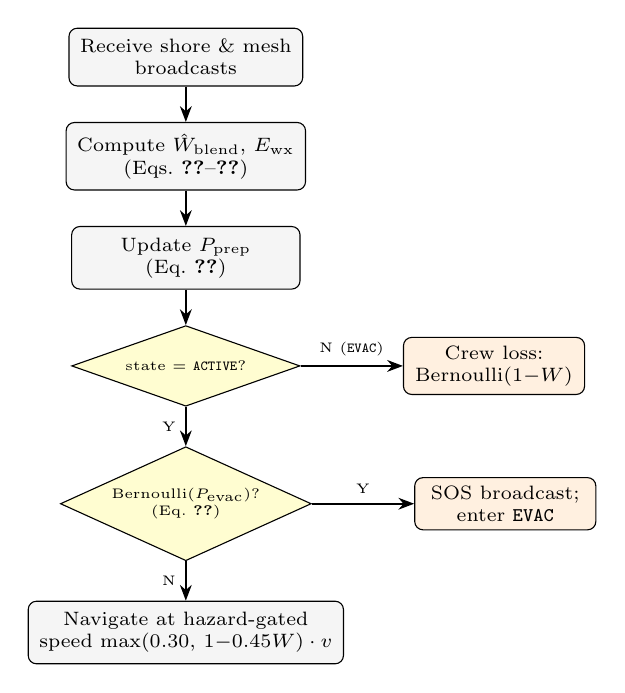
\begin{tikzpicture}[
  >=Stealth, font=\scriptsize,
  node distance=0.45cm and 1.3cm,
  proc/.style={draw, rounded corners=3pt, fill=gray!8,
               minimum width=2.9cm, minimum height=0.60cm,
               align=center, inner sep=4pt},
  dec/.style={draw, diamond, shape aspect=2.2, fill=yellow!18,
              minimum width=2.9cm, align=center, inner sep=2pt, font=\tiny},
  alarm/.style={draw, rounded corners=3pt, fill=orange!12,
                minimum width=2.3cm, minimum height=0.60cm,
                align=center, inner sep=3pt},
  arr/.style={->, semithick},
]
  %% Main vertical path
  \node[proc] (recv) {Receive shore \& mesh\\broadcasts};
  \node[proc, below=of recv] (fuse) {Compute $\hat{W}_\text{blend}$, $E_\text{wx}$\\(Eqs.~\ref{eq:confidence}--\ref{eq:blend})};
  \node[proc, below=of fuse] (prep) {Update $P_\text{prep}$\\(Eq.~\ref{eq:Pprep})};
  \node[dec,  below=of prep] (stateq) {state $=$ \texttt{ACTIVE}?};
  \node[dec,  below=0.5cm of stateq] (evacq) {Bernoulli$(P_\text{evac})$?\\(Eq.~\ref{eq:evac})};
  \node[proc, below=0.5cm of evacq] (nav) {Navigate at hazard-gated\\speed $\max(0.30,\,1{-}0.45W)\cdot v$};

  %% Right-side branches
  \node[alarm, right=1.3cm of stateq] (crew)
    {Crew loss:\\Bernoulli$(1{-}W)$};
  \node[alarm, right=1.3cm of evacq] (sos)
    {SOS broadcast;\\enter \texttt{EVAC}};

  %% Arrows — main path
  \draw[arr] (recv)   -- (fuse);
  \draw[arr] (fuse)   -- (prep);
  \draw[arr] (prep)   -- (stateq);
  \draw[arr] (stateq) -- node[left, font=\tiny]{Y} (evacq);
  \draw[arr] (evacq)  -- node[left, font=\tiny]{N} (nav);

  %% Arrows — branches
  \draw[arr] (stateq.east) -- node[above, font=\tiny]{N (\texttt{EVAC})} (crew.west);
  \draw[arr] (evacq.east)  -- node[above, font=\tiny]{Y} (sos.west);
\end{tikzpicture}
\caption{Per-tick behavioural pipeline for every \texttt{VesselAgent} (macro-tick step~5). Shore and mesh inboxes are fused into $\hat{W}_\text{blend}$, from which $P_\text{prep}$ is derived. An \texttt{ACTIVE} vessel then samples the evacuation probability; failure to trigger leads to hazard-gated navigation while a positive draw broadcasts SOS and opens the rescue pipeline. Vessels already in \texttt{EVAC} bypass the decision branch and lose crew members each tick until rescue arrives.}
\label{fig:vessel-pipeline}
\end{figure}

\subsection{Human Factors and Preparedness Score}

Crew error probability integrates accumulated fatigue and the circadian rhythm of human vigilance. The circadian component is modelled as a negated cosine that reaches its minimum at 03:00~UTC — the well-documented performance nadir of watch-keepers~\cite{chauvin2013} — and its maximum at 15:00~UTC. The phase offset $\phi_\text{nadir} = 3$ (hours UTC) locates that trough:
%
\begin{equation}
  F_\text{circ} = -\cos\left(\tfrac{2\pi}{24}
                  (t_\text{utc} - \phi_\text{nadir})\right).
  \label{eq:circadian}
\end{equation}
%
Combining fatigue, circadian phase, and crew archetype into a single error probability:
%
\begin{equation}
  P_\text{err} = \sigma\left(
    w_a\cdot\texttt{hours\_awake}
    + w_c\cdot F_\text{circ}
    + \text{Arch\_Mod} - B_c
  \right),
  \label{eq:Perr}
\end{equation}
%
with $w_a = 0.12$, $w_c = 1.5$, $B_c = 4.0$, and archetype modifiers of $-1.5$ (Veteran), $0.0$ (Standard), and $+2.0$ (Green crew). Higher $P_\text{err}$ reflects a more error-prone watch. Archetype assignment at spawn follows a two-stage draw: with probability \texttt{green\_crew\_fraction} the vessel is assigned \textsc{Green}, otherwise \textsc{Standard}; a second independent draw then promotes 10\,\% of all vessels to \textsc{Veteran} regardless of the first outcome.

The \emph{preparedness score} $P_\text{prep} \in [0,1]$ captures how well a vessel is positioned to respond to hazards, penalising both forecast inaccuracy and a high-risk crew archetype:
%
\begin{equation}
  P_\text{prep} = \text{clip}\left(
    1 - \eta\,E_\text{wx} - \xi\,\text{Arch\_Mod},\,0,\,1
  \right),
  \label{eq:Pprep}
\end{equation}
%
with $\eta = 1.5$ and $\xi = 0.2$. $P_\text{prep}$ gates every tactical decision each tick: course alteration, speed reduction, and the evacuation trigger below. A veteran crew with a near-perfect blended forecast achieves $P_\text{prep} \approx 1$; inexperienced crew with large forecast error is driven toward zero.

\subsection{Early Evacuation Decision}

Each tick, a vessel first computes a baseline evacuation propensity:
%
\begin{equation}
  P_\text{evac,raw} = \sigma\left(
    b_0
    +
    \alpha\,\hat{W}_\text{blend}
    - \beta\,E_\text{wx}
    + \gamma\,P_\text{prep}
  \right),
  \label{eq:evac-raw}
\end{equation}
%
with $b_0=-2.8$, $\alpha = 4.0$, $\beta = 2.5$, $\gamma = 1.8$. To prevent unrealistic mass evacuations in the first few ticks, the hazard term is ramped by both time and severity:
%

\begin{align}
  &\hat{W}_\text{eff} = \hat{W}_\text{blend} \cdot r_t \cdot r_w, \\
  &r_t = \operatorname{clip}\left(\frac{t+1}{24},\,0.08,\,1\right), \\
  &r_w = \operatorname{clip}\left(\frac{\hat{W}_\text{blend}}{0.75},\,0.10,\,1\right),
  \label{eq:evac-ramp}
\end{align}
%
and the final Bernoulli trigger uses:
%
\begin{equation}
  P_\text{evac} = \sigma\left(
    b_0
    + \alpha\,\hat{W}_\text{eff}
    - \beta\,E_\text{wx}
    + \gamma\,P_\text{prep}
  \right),
  \label{eq:evac}
\end{equation}
%
A high effective hazard estimate and high preparedness score promote evacuation; large forecast error suppresses it, preventing false alarms in noisy information conditions. This preserves hazard sensitivity while damping early-tick false positives. On trigger, the vessel broadcasts an SOS packet and begins raft deployment.

\subsection{Raft Deployment and Post-Incident Survival}

Whether a life-raft deploys successfully depends on both current weather severity and how prepared the crew is:
%
\begin{equation}
  P_\text{raft} = \text{clip}\left(
    B_\text{raft} - \delta_\text{wx}\,W + \delta_\text{prep}\,P_\text{prep},
    \,0,\,1\right),
  \label{eq:raft}
\end{equation}
%
with $B_\text{raft} = 0.90$, $\delta_\text{wx} = 0.60$, $\delta_\text{prep} = 0.25$. Once in rafts, crew members remain exposed until rescue arrives. Time-to-Arrival (TTA) is:
%
\begin{equation}
  \text{TTA} = \frac{d_\text{ship,dispatch-station}}{v_\text{rescue} \cdot \max(0.40,\,1-0.35\,W)}
               + \Delta t_\text{mob},
  \label{eq:tta}
\end{equation}
%
where $v_\text{rescue} \in \{80\,\text{kn (helicopter)},\,25\,\text{kn (patrol vessel)}\}$ with equal dispatch probability, $\Delta t_\text{mob} = 2$ ticks for mobilisation, and the denominator captures a weather-dependent speed reduction applied to the rescue asset in transit. Survivor probability per raft-tick decreases as $1 - W$ (Bernoulli draw per crew member per tick), so evacuating earlier — when $W$ is still moderate — directly improves survival. This is the causal mechanism behind H2: better mesh coverage $\to$ lower $E_\text{wx}$ $\to$ higher $P_\text{prep}$ $\to$ earlier evacuation $\to$ lower $W$ at evacuation time $\to$ higher survival.

\subsection{Collision and Grounding Detection}

Ship--ship collisions are detected using pairwise circle-overlap checks: each vessel occupies a disc of radius $r = 0.15$\,nm, consistent with near-miss studies on vessel encounter geometry~\cite{zhang2015}, and two vessels collide when their centre-to-centre distance falls within $2r = 0.30$\,nm. Each collision increments both vessels' damage counters; a vessel transitions to \texttt{SUNK} once its damage counter reaches the \texttt{stability\_threshold} of~3, incrementing the fatality counter (KPI~1, Table~\ref{tab:kpis}).

In addition, land collisions (groundings) are detected by testing vessel motion segments against the land mask each tick. On grounding, the vessel is moved back to its last valid water position (avoidance effect), damage is incremented, and the state transitions to \texttt{EVAC}, initiating the same rescue/SOS workflow as for severe ship incidents. Groundings are logged as intervention events for map playback and KPI accounting.

% ==================================================================
\section{Experimental Design}
\label{sec:experiment}
% ==================================================================

This section defines the experimental conditions, scenarios, KPIs, and statistical analysis methods used to test the hypotheses. The weather engine is configured through a two-level GUI scheme: \emph{Basic} presets (\texttt{calm}, \texttt{mixed}, \texttt{stormy}) for fast setup and \emph{Advanced} controls exposing the full Tier-2 parameter set.

\subsection{Methods Under Test}

The three experimental conditions introduced in Section~\ref{sec:goal} are formally defined as follows:

\begin{itemize}[leftmargin=1.2em, itemsep=2pt]
    \item \textbf{Baseline~A (Classical):} No weather intelligence; no preparedness modifier; deterministic COLREGs navigation only. $P_\text{prep} \equiv 0$ throughout.
    \item \textbf{Baseline~B (Shore-Only):} Shore forecast received via Eqs.~\ref{eq:shoreNoise}--\ref{eq:Prx} when in range; no mesh relay; no confidence fusion. Shore-trust decay constant is set to $k_\lambda \to 0$, making $\lambda_\text{ship} \to 1$ immediately after any missed shore reception; since mesh is disabled and $\hat{W}_\text{ship} = \varnothing$, the fuser falls back to $\hat{W}_\text{blend} \equiv \hat{W}_\text{shore}$ whenever shore data is available, and to $\hat{W}_\text{blend} = 0$ when out of range.
    \item \textbf{Proposed System:} Full pipeline — Eqs.~\ref{eq:shoreNoise}--\ref{eq:blend} for forecast fusion, Eqs.~\ref{eq:Pprep}--\ref{eq:raft} for behaviour, and hop-limited SOS relay.
\end{itemize}

An ablation matrix additionally disables each component in turn: mesh off ($\lambda_\text{ship} \equiv 0$), evacuation off ($P_\text{evac} \equiv 0$), human factors off ($P_\text{err} \equiv 0$).

\subsection{Scenarios}

Table~\ref{tab:scenarios} summarises the four scenarios. All share the same $100 \times 100$\,nm world; each is implemented as a factory function that configures the model constructor with no scenario-specific branching inside agent code. Each scenario specifies weather-regime and storm-system settings in addition to communication and noise stressors, and runs 30 independent seeds.

Each simulation run uses $n_\text{ticks}=2880$ with a 15\,min macro tick (Section~\ref{sec:model}), so one run covers $720$\,h ($30$ days). With three methods (Baseline~A, Baseline~B, Proposed) and four scenarios, the full experiment plan executes $4 \times 3 \times 30 = 360$ runs.

\begin{table*}[htbp]
    \caption{Scenario summary. $\sigma_\text{shore}$ is shore forecast standard deviation. All scenarios use 30 seeds and 2880 ticks/run (30 days at 15\,min/tick).}
    \label{tab:scenarios}
    \centering
    \small
    \begin{tabularx}{\textwidth}{@{}l>{\raggedright\arraybackslash}Xccr@{}}
        \toprule
        Scenario & Key conditions & Ships & Duration & Hyp. \\
        \midrule
        1 — Calm Passage &
        calm-biased weather, $\sigma_\text{shore}{=}0.05$, 10\,\% Green crew.
        Pass: ${<}0.5$ collisions per 1\,k ship-hrs. &
        20 & 30 d &
        Calib. \\[4pt]
        2 — Storm Corridor &
        storm-focused weather; $\sigma_\text{shore}{=}0.18$;
        30\,\% Green crew. &
        25 & 30 d &
        H1 \\[4pt]
        3 — Blind Shore &
        offshore spawn annulus 40--70\,nm; 30\,\% Green crew;
        $\sigma_\text{shore}$ doubles to $0.36$ at tick~40. &
        25 & 30 d &
        H3 \\[4pt]
        4 — Deep Water Rescue &
        offshore spawn annulus 60--100\,nm; 25\,\% Green crew;
        $W$ spikes to 0.90 at grid centre (tick~30). &
        15 & 30 d &
        H2, H3 \\
        \bottomrule
    \end{tabularx}
\end{table*}

\subsection{Key Performance Indicators}

Table~\ref{tab:kpis} defines the six KPIs collected per run. KPIs~1--2 test H1, KPIs~3--5 test H2, and KPI~6 tests H3. All are computed from per-tick logs flushed incrementally to Parquet chunks during execution, then aggregated for analysis, ensuring reproducibility while avoiding high in-memory retention on long runs.

\begin{table}[htbp]
    \caption{KPI definitions and hypothesis links. \textit{ship-hrs} $=$ total agent-hours in \texttt{ACTIVE} or \texttt{EVAC} state.}
    \label{tab:kpis}
    \centering
    \small
    \begin{tabularx}{\columnwidth}{@{}clXc@{}}
        \toprule
        \# & KPI & Definition & Hyp. \\
        \midrule
        1 & \texttt{fatal\_per\_1k\_hrs}
        & Fatal events $\div$ ship-hrs $\times 10^3$
        & H1 \\
        2 & \texttt{collision\_per\_1k\_hrs}
        & Collision events $\div$ ship-hrs $\times 10^3$
        & H1 \\
        3 & \texttt{survival\_ratio}
        & Survivors\,/\,(survivors + fatalities)
        & H2 \\
        4 & \texttt{avg\_tta\_hours}
        & Mean rescue Time-to-Arrival across dispatches
        & H2 \\
        5 & \texttt{evac\_activation\_rate}
        & Fraction of vessels that triggered early evac.
        & H2, H3 \\
        6 & \texttt{mean\_p\_prep}
        & Time-averaged $P_\text{prep}$ across all vessels
        & H3 \\
        \bottomrule
    \end{tabularx}
\end{table}

\subsection{Statistical Analysis}

Hypothesis decisions use the Mann-Whitney U test --- appropriate for the bounded, non-normal KPI distributions produced by a finite-agent simulation. Effect sizes are reported as Cliff's $\Delta$~\cite{cliff1993}; both $p < 0.05$ and $\Delta > 0.2$ (small effect) are required for H1 and H3 to be confirmed. Confidence intervals are bootstrapped over the 30 seeds. The same seed sequence is applied to all conditions to eliminate seed-selection bias from pairwise comparisons. For each run, the full effective weather parameter set and seed are written to the manifest, enabling byte-level replay and sensitivity sweeps over the weather process.

\subsection{Operational Hyperparameters and Runtime Profile}

Beyond scenario-level stressors, the engine exposes a complete set of run-control hyperparameters in the GUI and run manifest. This enables direct auditability of experiment context and supports long-horizon what-if studies without changing agent logic.

\begin{table*}[htbp]
    \caption{Operational hyperparameters used in configured runs.}
    \label{tab:operational-hparams}
    \centering
    \small
    \begin{tabularx}{16cm}{@{}lX@{}}
        \toprule
        Hyperparameter & Value / role \\
        \midrule
        \texttt{n\_vessels} & Fleet size per run; the stress profile supports up to 100 concurrent vessels. \\
        \texttt{n\_ticks} & Simulation horizon. At 15\,min/tick, month-long runs use 2880 ticks. \\
        \texttt{n\_seeds} & Number of independent stochastic repetitions per method/scenario pair. \\
        \texttt{world\_size\_nm} & Physical map extent (default 100$\times$100\,nm). \\
        \texttt{min/max\_spawn\_distance\_nm} & Endpoint-centred spawn annulus bounds controlling offshore traffic initialisation. \\
        \texttt{lane\_endpoint\_spawn\_weights} & Per-route endpoint sampling weights shaping directional traffic density. \\
        \texttt{vessel\_radio\_range\_nm}, \texttt{max\_hop\_count} & Mesh communication reach and relay depth. \\
        \texttt{shore\_broadcast\_radius\_nm} & Shore coverage radius (default 50\,nm). \\
        \texttt{radio\_packet\_loss\_rate} & Stochastic packet-drop probability (default 2\,\%). \\
        Weather Tier-2 parameters & Regime transitions, storm spawning, system geometry, drift, persistence, coupling, shocks, and hazard-channel weights. \\
        \bottomrule
    \end{tabularx}
\end{table*}

To maintain stable exposure over long horizons, terminal vessel states (\texttt{SUNK}, \texttt{RESCUED}) are recycled in-engine: agents are removed from the scheduler, replaced with freshly spawned vessels, and the active population is restored to the configured \texttt{n\_vessels} target each tick. This keeps month-long high-density runs analytically comparable across methods despite attrition.

% ==================================================================
\section{Implementation}
\label{sec:implementation}
% ==================================================================

The preceding sections describe the model in terms of protocols and equations. This section covers how the engine executes them: the per-tick computation order, the weather update pipeline, relay mechanics, vessel navigation, and the rescue workflow. The description is self-contained enough to reimplement or extend any component independently.

\subsection{Simulation Loop}
\label{sec:loop}

Every run executes 2\,880 macro ticks (30 days at 15\,min each). Within each tick, computation runs in four sequential phases — Fig.~\ref{fig:tick-loop} — whose ordering is a causal constraint, not a convention. Shore stations broadcast before vessels step, so a vessel's blended forecast in tick $t$ already incorporates the shore estimate issued in that same tick. The relay phase runs immediately after broadcasting: a vessel that enters \texttt{EVAC} mid-tick has its SOS forwarded to shore and rescue dispatched within the same 15-minute window, bounding mobilisation latency to exactly one macro tick. The full 11-step breakdown appears in Appendix~\ref{apx:tick}.

The two stochastic hazard events — a hazard spike at tick $t_\text{spike}$ and shore-noise doubling at tick $t_\text{noise}$ — fire at the top of the weather phase, before any agent step, so all agents face the modified field simultaneously on the configured tick.

\begin{figure}[htbp]
\centering
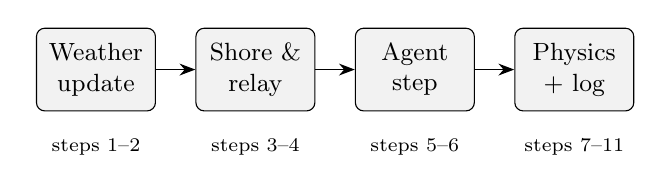
\begin{tikzpicture}[
  >=Stealth, font=\small,
  ph/.style={draw, rounded corners=3pt,
             minimum width=1.42cm, minimum height=1.05cm,
             align=center, fill=gray!10, text width=1.3cm, inner sep=3pt},
  arr/.style={->, semithick},
  lbl/.style={font=\scriptsize, text width=1.5cm, align=center},
  node distance=0.5cm,
]
  \node[ph] (w) {Weather\\update};
  \node[ph, right=of w] (c) {Shore \&\\relay};
  \node[ph, right=of c] (a) {Agent\\step};
  \node[ph, right=of a] (p) {Physics\\+\ log};
  \draw[arr] (w) -- (c);
  \draw[arr] (c) -- (a);
  \draw[arr] (a) -- (p);
  \node[lbl, below=0.22cm of w] {steps 1--2};
  \node[lbl, below=0.22cm of c] {steps 3--4};
  \node[lbl, below=0.22cm of a] {steps 5--6};
  \node[lbl, below=0.22cm of p] {steps 7--11};
\end{tikzpicture}
\caption{Four computational phases of each macro tick. Data flows strictly left to right within a tick; no agent reads results produced later in the same phase. Full step list in Appendix~\ref{apx:tick}.}
\label{fig:tick-loop}
\end{figure}

\subsection{Weather Process}
\label{sec:weather-impl}

A uniform random hazard field would not produce the spatial divergence between shore conditions and offshore reality that makes peer weather-sharing valuable in the first place. The Tier-2 process generates localised storm cells, coherent fronts, and realistic channel co-variation, while remaining light enough for interactive simulation on a laptop.

Each tick the $50\times50$ grid is updated in seven ordered stages.

\begin{itemize}[leftmargin=*, itemsep=2pt]
    \item \textbf{Regime switch.} A Bernoulli draw may flip the global regime: calm$\to$storm at probability $p_{cs}$ (default 0.03), storm$\to$calm at probability $p_{sc}$ (default 0.08). For the \texttt{calm} preset, the transition kernel is additionally damped ($p_{cs}\times0.35$, $p_{sc}\times1.4$) to avoid unrealistically fast escalation.

    \item \textbf{Storm cell lifecycle.} Up to \texttt{max\_systems} circular cells may be active. Each tick a new cell may spawn at probability $p_\text{spawn}\times r_\text{regime}$ ($r=1.35$ in storm, $0.65$ in calm by default). For the \texttt{calm} preset this boost is reduced further (storm 0.75, calm 0.20), and overlay/coupling/shock amplitudes are down-scaled to preserve calm persistence. Active cells drift at 0.6 grid-cells/tick along a jittered bearing; radius oscillates sinusoidally; intensity decays faster in calm (0.020/tick) than in storm (0.006/tick). Cells below intensity 0.12 are removed.

    \item \textbf{Background AR(1) evolution.} Each channel evolves with advection and mean-reversion:
    \begin{equation}
      X_{t+1} = \rho_X\,\mathrm{adv}(X_t)
                 + (1-\rho_X)\,\mu_X
                 + \sigma_X(0.3+u)\,\eta_t,
      \label{eq:ar1}
    \end{equation}
    where $\mathrm{adv}(\cdot)$ shifts the grid by a slowly drifting integer offset $(-1,0,{+}1)$ cells per axis, $\rho_X$ is per-channel persistence, $\mu_X$ is the mean-reversion target, $\sigma_X$ is innovation scale, and $u\in[0,1]$ is the scenario unpredictability parameter. Default values: $\rho_s{=}0.95$, $\rho_v{=}0.90$, $\rho_u{=}0.93$; $\mu_s{=}\mu_u{=}0.5$, $\mu_v{=}0.7$ (visibility baseline is fair-weather). The persistence values place the effective response timescale at 15--20 ticks (3--5 hours) for sea state and 10--12 ticks for visibility and wind, consistent with observed mesoscale forcing response.

    \item \textbf{System overlay.} Each active cell's Gaussian kernel — intensity-weighted in sea and wind, negated in visibility — is added on top of the background, so a storm cell simultaneously elevates seas, strengthens winds, and cuts sight lines.

    \item \textbf{Cross-channel coupling.}
    \begin{align}
      s &\mathrel{+}= 0.35(u-0.5) \\
      s &\mathrel{-}= 0.20(v-0.5) \\
      u &\mathrel{-}= 0.25(v-0.5)
      \label{eq:coupling}
    \end{align}
    High wind drives sea state up and visibility down; high visibility implies moderate wind and calm seas. The signs and magnitudes reproduce the co-variation structure seen in ERA5 reanalysis data over the North Atlantic.

    \item \textbf{Front structure.} A sinusoidal plane wave aligned with the prevailing drift direction adds elongated spatial structure, producing coherent frontal gradients absent from any purely circular model.

    \item \textbf{Shocks, smoothing, and gradient limiting.} With probability $p_\text{shock}(0.3+u)$ (default 1.5\,\% at $u{=}0$), a spatially correlated Gaussian shock hits all three channels simultaneously (sea $\times 1.0$, wind $\times 0.8$, visibility $\times -0.6$), modelling a sudden squall. A 5-point neighbourhood smoother followed by a gradient limiter (maximum cell-to-cell change 0.12) then enforces spatial coherence.
\end{itemize}

\subsection{Agent Communication}
\label{sec:relay-impl}

\begin{figure*}[t]
\centering
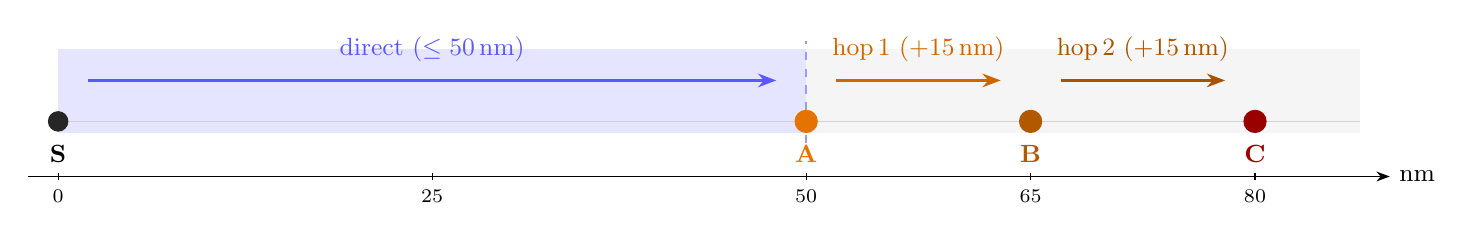
\begin{tikzpicture}[x=0.19cm, >=Stealth]
  %% Background zones — no text inside; caption explains the shading
  \fill[blue!10] (0,-0.15) rectangle (50, 0.92);
  \fill[gray!8]  (50,-0.15) rectangle (87, 0.92);
  \draw[blue!40, dashed, thick] (50,-0.28) -- (50, 1.02);

  %% Relay arrows — sole occupants of their horizontal band (y = 0.52)
  \draw[->, thick, blue!65] (2, 0.52) -- (48, 0.52)
    node[midway, above=3pt, font=\small]{direct ($\leq 50$\,nm)};
  \draw[->, thick, orange!80!black] (52, 0.52) -- (63, 0.52)
    node[midway, above=3pt, font=\small]{hop\,1 ($+15$\,nm)};
  \draw[->, thick, orange!65!black] (67, 0.52) -- (78, 0.52)
    node[midway, above=3pt, font=\small]{hop\,2 ($+15$\,nm)};

  %% Centre line
  \draw[gray!35, thin] (0,0) -- (87,0);

  %% Station and vessel dots — labels placed below, away from arrows
  \filldraw[black!85] (0,0) circle (3.5pt);
  \node[below=5pt, font=\small\bfseries] at (0,0) {S};

  \filldraw[orange!90!black] (50,0) circle (4pt);
  \node[below=5pt, font=\small\bfseries, orange!90!black] at (50,0) {A};

  \filldraw[orange!70!black] (65,0) circle (4pt);
  \node[below=5pt, font=\small\bfseries, orange!70!black] at (65,0) {B};

  \filldraw[red!60!black] (80,0) circle (4pt);
  \node[below=5pt, font=\small\bfseries, red!60!black] at (80,0) {C};

  %% X-axis — well below the vessel labels
  \draw[->] (-2,-0.70) -- (89,-0.70) node[right, font=\small]{nm};
  \foreach \x in {0,25,50,65,80}
    \draw (\x,-0.65) -- (\x,-0.75) node[below, font=\scriptsize]{\x};
\end{tikzpicture}
\caption{Two-hop relay coverage (blue\,=\,shore zone $\leq 50$\,nm; gray\,=\,radio shadow). Shore station~S broadcasts directly within 50\,nm. Vessel~A (at the boundary) relays its local weather observation to~B (hop\,1, $+15$\,nm), which relays to~C (hop\,2, $+15$\,nm), extending effective data reach to 80\,nm — 30\,nm beyond the shore horizon. \texttt{max\_hop\_count}\,=\,2 suppresses a third relay.}
\label{fig:relay}
\end{figure*}

Fig.~\ref{fig:relay} makes the two-hop design choice concrete. Shore covers the coastal band to 50\,nm. Each relay hop adds 15\,nm, so two hops extend the horizon to 80\,nm — comfortably covering the offshore spawn zones of Scenarios~3 and~4. A third hop would add another 15\,nm but at the cost of data already three ticks old by the time a vessel acts on it, plus a relay fanout that grows quadratically with fleet density per tick. Two hops is the configuration where coverage gain and communication overhead balance.

The relay engine runs after shore broadcast and before vessel behaviour. It iterates over all active vessels in a single pass. A packet is forwarded only if (a)~the hop count is below \texttt{max\_hop\_count} and (b)~the recipient has not seen this packet yet in the current tick. Without condition~(b), a fleet of 25 vessels would generate a relay fanout growing exponentially with vessel count per tick.

SOS packets share the relay queue but with priority routing: the engine first attempts direct delivery to every shore station within radio range (via Eq.~\ref{eq:Prx}). Relay to other vessels fires only when all direct attempts fail, so rescue dispatch is bounded to one tick for any vessel connected to shore through a relay chain.

\subsection{Vessel Navigation}
\label{sec:nav-impl}

Vessels use an ordered-waypoint traveller with a per-tick distance budget of $v\cdot\max(0.30,\,1-0.45\,W)\cdot\Delta t$, where $v\sim\mathcal{U}(10,20)$\,kn is drawn at spawn and $W$ is the current local hazard. Budget is consumed incrementally against the vector to the current target waypoint; on arrival the index advances and wraps at the last waypoint, so the route is traversed continuously in alternating directions.

Before committing any move, the engine tests whether the proposed segment intersects the land mask. If it does, the step distance is halved up to four times to find the largest safe sub-step. When no safe sub-step is found — typically when a vessel approaches a headland nearly head-on — the target index advances and the vessel holds position for the tick. This two-level fallback is sufficient for the five default routes, which are designed to avoid geometric dead-ends under this algorithm.

Active collision avoidance is not modelled; the hazard-gated speed reduction acts as an implicit braking mechanism. A well-prepared crew slows in deteriorating weather, reducing closing rates on converging lanes. The causal chain of interest runs through \emph{information quality}, not through evasion geometry, so adding explicit COLREGs manoeuvring logic would obscure rather than test the central hypothesis.

\subsection{Rescue Pipeline}
\label{sec:rescue-impl}

\begin{figure}[htbp]
\centering
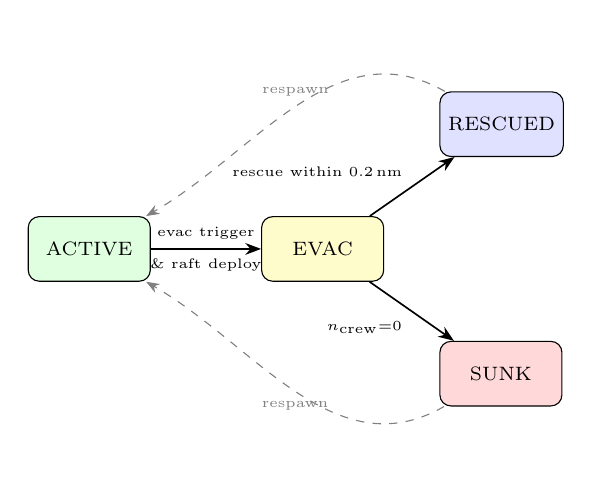
\begin{tikzpicture}[
  >=Stealth, font=\scriptsize,
  st/.style={draw, rounded corners=4pt, minimum width=1.55cm, minimum height=0.82cm,
             align=center, inner sep=3pt},
  arr/.style={->, semithick},
  node distance=0.95cm and 1.4cm,
]
  \node[st, fill=green!12]  (A) {ACTIVE};
  \node[st, fill=yellow!20, right=of A] (E) {EVAC};
  \node[st, fill=red!15,  below right=0.75cm and 0.7cm of E] (S) {SUNK};
  \node[st, fill=blue!12, above right=0.75cm and 0.7cm of E] (R) {RESCUED};
  \draw[arr] (A) -- node[above, font=\tiny]{evac trigger}
                    node[below, font=\tiny]{\& raft deploy} (E);
  \draw[arr] (E) -- node[below left, font=\tiny]{$n_\text{crew}{=}0$} (S);
  \draw[arr] (E) -- node[above left, font=\tiny]{rescue within 0.2\,nm} (R);
  \draw[->, dashed, gray] (S) to[out=-150, in=-30]
      node[below, font=\tiny, gray]{respawn} (A);
  \draw[->, dashed, gray] (R) to[out=150, in=30]
      node[above, font=\tiny, gray]{respawn} (A);
\end{tikzpicture}
\caption{Vessel state machine. Dashed arrows show the respawn loop: terminal agents are removed at tick end and replaced with fresh vessels at sampled lane endpoints, keeping fleet size constant at \texttt{n\_vessels}.}
\label{fig:fsm}
\end{figure}

Fig.~\ref{fig:fsm} shows the complete vessel state machine. A vessel transitions to \texttt{EVAC} when the evacuation policy fires and the raft deploys successfully (Eq.~\ref{eq:raft}), then loses crew members each tick at rate $1-W$ until all survivors are gone (\texttt{SUNK}) or a rescue agent arrives within 0.2\,nm (\texttt{RESCUED}). The 0.2\,nm threshold models the physical reach of a helicopter hoist or liferaft pickup in moderate sea state; both terminal states trigger an immediate respawn to maintain fleet size.

When a vessel first enters \texttt{EVAC} the relay engine routes its SOS toward shore. The first coastal station to successfully receive it (Eq.~\ref{eq:Prx}) becomes the dispatch origin — reflecting the real practice that the station receiving the Mayday coordinates the response. The engine then spawns one rescue asset: helicopter (80\,kn) with 50\,\% probability, patrol vessel (25\,kn) otherwise, matching a typical mixed SAR resource deployment~\cite{imosar2018}. Both asset types wait 2 ticks for mobilisation before navigating directly to the last known distress position at $v_\text{rescue}\cdot\max(0.40,\,1-0.35\,W)$ kn. Each crew member of the rescued vessel survives independently; $n_\text{crew}=10$ per vessel. Fig.~\ref{fig:seq} traces this pipeline as a UML sequence diagram.

\begin{figure*}[t]
\centering
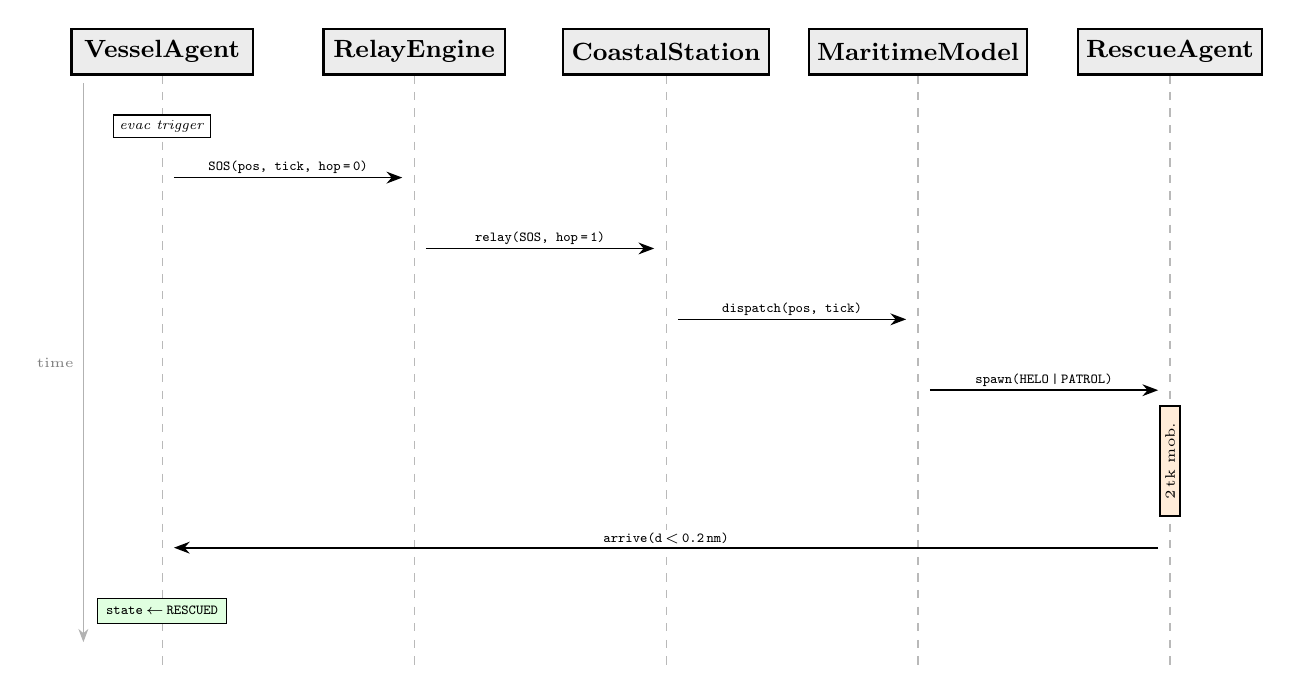
\begin{tikzpicture}[
  >=Stealth, font=\scriptsize,
  actor/.style={draw, thick, fill=gray!15,
                minimum width=2.3cm, minimum height=0.58cm,
                align=center, font=\small\bfseries, inner sep=3pt},
  msg/.style={->, semithick},
  lf/.style={dashed, gray!55, thin},
  nm/.style={font=\tiny, fill=white, inner sep=1pt},
]
  %% Lifelines (drawn first, behind everything else)
  \foreach \x in {0, 3.2, 6.4, 9.6, 12.8}
    \draw[lf] (\x, -0.30) -- (\x, -7.8);

  %% Actor boxes
  \node[actor] at (0,    0) {VesselAgent};
  \node[actor] at (3.2,  0) {RelayEngine};
  \node[actor] at (6.4,  0) {CoastalStation};
  \node[actor] at (9.6,  0) {MaritimeModel};
  \node[actor] at (12.8, 0) {RescueAgent};

  %% EVAC trigger annotation
  \node[draw, fill=white, font=\tiny, inner sep=2pt] at (0, -0.95)
    {\textit{evac trigger}};

  %% Message 1: VesselAgent → RelayEngine
  \draw[msg] (0.15, -1.6) -- (3.05, -1.6)
    node[nm, above, midway]{\texttt{SOS(pos, tick, hop\,=\,0)}};

  %% Message 2: RelayEngine → CoastalStation
  \draw[msg] (3.35, -2.5) -- (6.25, -2.5)
    node[nm, above, midway]{\texttt{relay(SOS, hop\,=\,1)}};

  %% Message 3: CoastalStation → MaritimeModel
  \draw[msg] (6.55, -3.4) -- (9.45, -3.4)
    node[nm, above, midway]{\texttt{dispatch(pos, tick)}};

  %% Message 4: MaritimeModel → RescueAgent
  \draw[msg] (9.75, -4.3) -- (12.65, -4.3)
    node[nm, above, midway]{\texttt{spawn(HELO\,|\,PATROL)}};

  %% RescueAgent activation: 2-tick mobilisation
  \draw[thick, fill=orange!15] (12.67, -4.5) rectangle (12.93, -5.9);
  \node[font=\tiny, rotate=90] at (12.8, -5.2) {2\,tk mob.};

  %% Message 5: RescueAgent → VesselAgent (return arrow)
  \draw[msg] (12.65, -6.3) -- (0.15, -6.3)
    node[nm, above, midway]{\texttt{arrive(d\,$<$\,0.2\,nm)}};

  %% RESCUED state annotation
  \node[draw, fill=green!12, font=\tiny, inner sep=3pt] at (0, -7.1)
    {\texttt{state\,$\leftarrow$\,RESCUED}};

  %% Time axis
  \draw[->, gray!60, thin] (-1.0, -0.4) -- (-1.0, -7.5)
    node[midway, left, font=\tiny, gray]{time};
\end{tikzpicture}
\caption{UML sequence diagram for the SOS and rescue pipeline. On entering \texttt{EVAC}, the vessel broadcasts an SOS hop\,=\,0 packet; the relay engine routes it to shore within the current 15\,min tick. The coastal station dispatches and \texttt{MaritimeModel} spawns a rescue asset. After a 2-tick (30\,min) mobilisation, the asset navigates to the distress position; arrival within 0.2\,nm transitions the surviving crew to \texttt{RESCUED}.}
\label{fig:seq}
\end{figure*}

% ==================================================================
\section{Results GUI}
\label{sec:results-gui}
% ==================================================================

The Streamlit dashboard provides an analysis workflow designed around experimental decision-making rather than static metric inspection. The lane-builder exposes a compact editor with explicit lane status badges, consolidated validation feedback, and resettable valid default routes.

The intended workflow is: (i) choose scenario and candidate methods on the \textit{Run} page, (ii) configure lane endpoints, per-endpoint spawn shares, and endpoint-centred spawn radii in the same GUI, (iii) rank methods by a selected KPI with confidence intervals and delta-to-baseline columns on the \textit{Results} page, (iv) confirm statistical significance in the \textit{Hypothesis} page using configurable method pairs, and (v) inspect representative seeds in \textit{Map Playback}. Setup and playback maps both render the active land mask and weather field; the setup map additionally visualises endpoint spawn annuli and communication ranges.

\subsection{Current limitations}
The GUI currently assumes schema-compatible outputs (\texttt{summary.csv}, per-run parquet, and run manifest version), and uncertainty is shown at KPI aggregate level only (no Bayesian posterior model). Future work should add richer event-level uncertainty decomposition and direct export of publication-ready figure bundles.

% ==================================================================
\section{Discussion}
\label{sec:discussion}
% ==================================================================

The target reference rate for calibration — fewer than 0.5 collisions per $1\,000$ ship-hours under Baseline~A in Scenario~1 (Table~\ref{tab:scenarios}) — is grounded in AIS-derived near-miss encounter statistics~\cite{silveira2013}. If H1 or H2 fail statistically, mitigation now includes recalibrating $(b_0,\alpha,\beta,\gamma)$ in Eq.~\ref{eq:evac-raw}, the ramp factors in Eq.~\ref{eq:evac-ramp}, or widening $\sigma_\text{shore}$ before final reporting; design parameters were chosen conservatively to make this adjustment feasible without invalidating the comparison.

The two-hop relay is sized deliberately: with a 15\,nm vessel radio range, two hops extend the effective data horizon by 30\,nm beyond the 50\,nm shore broadcast radius, reaching 80\,nm — sufficient to serve the spawn zones of Scenarios~3 and~4 (Table~\ref{tab:scenarios}). Removing the hop limit (unbounded flooding) would close any remaining gap trivially but obscure the protocol's practical value; the two-hop constraint models a real latency and battery trade-off in maritime IoT deployment.

The framework supports up to 100 concurrent vessels and month-long (2880 tick) runs, while retaining a $50 \times 50$ weather grid for map legibility and interactive dashboard performance on commodity hardware. Lane geometry, agent counts, run horizon, weather severity, and $\sigma_\text{shore}$ are all constructor parameters; additional experiment configurations can be added as factory functions without modifying any agent logic.

\bibliographystyle{IEEEtran}
\bibliography{mybib}

% ==================================================================
\appendix
% ==================================================================

\section{Macro-Tick Execution Sequence}
\label{apx:tick}

Table~\ref{tab:tick-steps} lists all eleven steps executed within each macro tick in the order they run. Steps 1--2 belong to the Weather phase, steps 3--4 to Communication, steps 5--6 to Agent behaviour, and steps 7--11 to Physics and housekeeping (see Fig.~\ref{fig:tick-loop} for the phase overview).

\begin{table*}[htbp]
    \caption{Complete macro-tick execution sequence.}
    \label{tab:tick-steps}
    \centering
    \small
    \begin{tabularx}{\textwidth}{@{}c l X@{}}
        \toprule
        \# & Phase & Action \\
        \midrule
        1 & Weather & Advance weather field: regime switch, storm cell lifecycle, AR(1) background evolution, system overlay, cross-channel coupling, front structure, shocks, smoothing, and gradient limiting. \\[2pt]
        2 & Weather & Apply scenario-scripted events: hazard spike at grid centre if \texttt{tick}~$= t_\text{spike}$; double shore-noise standard deviation if \texttt{tick}~$= t_\text{noise}$. \\[2pt]
        3 & Comms & Each coastal station samples local hazard, adds Gaussian noise (Eq.~\ref{eq:shoreNoise}), and probabilistically broadcasts to vessels in range (Eq.~\ref{eq:Prx}). \\[2pt]
        4 & Comms & Relay engine propagates weather packets and SOS queue; weather packets forwarded up to two hops; SOS routed to shore first, relayed only if shore is unreachable. \\[2pt]
        5 & Agents & Each vessel agent steps: reads shore and mesh inbox, computes confidence-weighted fusion (Eqs.~\ref{eq:confidence}--\ref{eq:blend}), updates preparedness (Eq.~\ref{eq:Pprep}), evaluates evacuation (Eq.~\ref{eq:evac}), and either navigates or loses crew. \\[2pt]
        6 & Agents & Each rescue agent decrements its mobilisation counter or advances toward the distress position at hazard-penalised speed. \\[2pt]
        7 & Physics & Pairwise ship--ship collision check over all \texttt{ACTIVE} vessels; damage counters incremented; vessels at threshold transition to \texttt{SUNK}. \\[2pt]
        8 & Physics & Motion-segment grounding check; groundings move the vessel back to its last valid water position, increment damage, and trigger \texttt{EVAC}. \\[2pt]
        9 & Physics & For each newly \texttt{RESCUED} vessel, record elapsed time since SOS dispatch as the TTA sample for \texttt{avg\_tta\_hours}. \\[2pt]
        10 & Housek. & Remove terminal vessels (\texttt{SUNK}, \texttt{RESCUED}) from the scheduler; spawn one fresh vessel per removed agent on a randomly sampled lane endpoint. \\[2pt]
        11 & Housek. & Append per-vessel and per-rescue state to the Parquet log; increment \texttt{tick}; advance simulation UTC clock by 0.25\,hr. \\
        \bottomrule
    \end{tabularx}
\end{table*}


\section{Default Constants Reference}
\label{apx:constants}

Table~\ref{tab:constants} lists every fixed constant defined in the engine with its default value and the design rationale. All values are accessible and overridable through \texttt{SimulationConfig}.

\begin{table*}[htbp]
    \caption{Engine default constants with design motivation. Values may be overridden via \texttt{SimulationConfig} or the dashboard GUI.}
    \label{tab:constants}
    \centering
    \small
    \begin{tabularx}{16cm}{@{}llX@{}}
        \toprule
        Constant & Default & Motivation \\
        \midrule
        \texttt{WORLD\_SIZE\_NM} & 100 & Large enough to place vessels beyond the 50\,nm shore horizon while keeping rendering interactive. \\
        \texttt{WEATHER\_GRID\_CELLS} & 50 & 2\,nm per cell; fine enough to resolve a storm cell smaller than a vessel's radio range, light enough for real-time rendering. \\
        \texttt{MACRO\_TICK\_HOURS} & 0.25 & 15\,min; matches AIS transponder reporting intervals and a typical COLREGs watch assessment period. \\
        \texttt{SHORE\_BROADCAST\_RADIUS\_NM} & 50 & Standard operational range for maritime MF/HF weather broadcasts. \\
        \texttt{SHORE\_NOISE\_MEAN} & 0.05 & Small positive bias; coastal stations tend to underestimate hazard in calm conditions relative to offshore reality. \\
        \texttt{SHORE\_NOISE\_STD\_NORMAL} & 0.18 & Produces a calibration collision rate below 0.5/1\,k ship-hrs under Baseline~A in Scenario~1. \\
        \texttt{SHORE\_NOISE\_STD\_STRESS} & 0.36 & Doubled noise for the H3 stress test; imposed at tick~40 in Scenario~3. \\
        \texttt{RADIO\_RANGE\_FALLOFF} ($\kappa_\text{radio}$) & 10 & Sigmoid scale giving a sharp reception edge at 50\,nm, with occasional long-range receptions under favourable propagation. \\
        \texttt{RADIO\_WEATHER\_INTERFERENCE} ($w_\text{intf}$) & 0.8 & Matches empirically observed radio degradation in Beaufort-7 conditions. \\
        \texttt{VESSEL\_RADIO\_RANGE\_NM} & 15 & Short-range VHF DSC horizon for a vessel with standard antenna height of $\sim$10\,m. \\
        \texttt{MAX\_HOP\_COUNT} & 2 & Point at which coverage gain (15\,nm/hop) balances data staleness and relay fanout growth. \\
        \texttt{FATIGUE\_WEIGHT} ($w_a$) & 0.12 & A crew awake for 24 hours adds $\approx 0.25$ to the error logit; comparable with accident-analysis findings~\cite{chauvin2013}. \\
        \texttt{CIRCADIAN\_WEIGHT} ($w_c$) & 1.5 & Produces a $\approx 15\,\%$ increase in $P_\text{err}$ at peak circadian impairment versus the well-rested baseline. \\
        \texttt{ERROR\_BIAS} ($B_c$) & 4.0 & Sets baseline $P_\text{err} \approx 0.02$ for a rested standard crew in calm conditions. \\
        \texttt{ARCHETYPE\_MOD\_VETERAN} & $-1.5$ & Reduces baseline $P_\text{err}$ to $\approx 0.008$. \\
        \texttt{ARCHETYPE\_MOD\_GREEN} & $+2.0$ & Raises baseline $P_\text{err}$ to $\approx 0.12$; reflects accident statistics for crews with fewer than two years of offshore experience. \\
        \texttt{PREP\_FORECAST\_ERROR\_PENALTY} ($\eta$) & 1.5 & A forecast error of 0.5 reduces $P_\text{prep}$ by 0.75, halving the vessel's tactical effectiveness. \\
        \texttt{PREP\_ARCHETYPE\_PENALTY} ($\xi$) & 0.2 & Green crews cannot fully recover preparedness even with perfect forecasts, reflecting skill limitations. \\
        \texttt{SHORE\_TRUST\_DECAY\_K} ($k_\lambda$) & 5 & Shore trust drops to $\approx 50\,\%$ after 5 ticks (75\,min) without a fresh reception; vessels at 60\,nm lose effective shore contact within about two hours of drifting into the shadow. \\
        \texttt{EVAC\_HAZARD\_WEIGHT} ($\alpha$) & 4.0 & Makes evacuation highly responsive to blended hazard above 0.5; logit exceeds 0 at $W_\text{blend} \approx 0.4$ for a prepared crew. \\
        \texttt{EVAC\_ERROR\_PENALTY} ($\beta$) & 2.5 & Suppresses evacuation when forecast error exceeds 0.4, preventing false alarms in noisy information conditions. \\
        \texttt{EVAC\_PREP\_WEIGHT} ($\gamma$) & 1.8 & Allows a fully prepared crew to evacuate at lower hazard thresholds than an unprepared one, quantifying the information-quality benefit. \\
        \texttt{EVAC\_BASELINE\_BIAS} ($b_0$) & $-2.8$ & Negative logit offset preventing mass immediate evacuations when hazards are still moderate at simulation start. \\
        \texttt{RAFT\_BASE\_SUCCESS} ($B_\text{raft}$) & 0.90 & 90\,\% baseline deployment success in calm conditions, matching manufacturer-reported reliability for modern inflatable liferafts. \\
        \texttt{RAFT\_WEATHER\_PENALTY} ($\delta_\text{wx}$) & 0.60 & Deployment probability drops to $\approx 30\,\%$ at $W{=}1$; severe seas make raft inflation and boarding hazardous. \\
        \texttt{RAFT\_PREP\_BONUS} ($\delta_\text{prep}$) & 0.25 & A well-prepared crew recovers up to 25\,\% of the weather penalty through drills and readiness. \\
        \texttt{HELICOPTER\_SPEED\_KN} & 80 & Standard SAR helicopter cruise speed (e.g., Sikorsky S-92)~\cite{imosar2018}. \\
        \texttt{PATROL\_VESSEL\_SPEED\_KN} & 25 & Representative of RNLI all-weather lifeboats and coastguard fast-response craft. \\
        \texttt{RESCUE\_MOBILISATION\_TICKS} & 2 & 30\,min mobilisation delay; accounts for crew scramble, pre-flight checks, and departure clearance. \\
        \texttt{COLLISION\_RADIUS\_NM} ($r$) & 0.15 & Vessels modelled as discs of radius 0.15\,nm; collision triggered when centres are within $2r{=}0.30$\,nm, consistent with AIS near-miss encounter geometry~\cite{zhang2015}. \\
        \bottomrule
    \end{tabularx}
\end{table*}

\end{document}
